\chapter{Thermodynamic assessment of redox controls on bacteriohopanepolyol headgroups}\label{ch3}


\section{Introduction}
Intro

BHP headgroups, also known as `side-chains', have been shown to situate in lipid bilayers facing outward (ref).


However, rather than using hypothetical site-average lipid structures, this study 

\section{Methods}

\subsection{Water chemistry and metering}
Methods used to meter, collect, and analyze water samples are described in Chapter \ref{ch1} and \ref{2}. Briefly, temperature was metered with a YSI 30 conductivity meter and pH with a model 3300i or 3110 WTW pH meter with WTW probe. A Hach model 2400 or 2800 portable spectrophotometer and Hach reagents/protocols were used to measure concentrations of dissolved oxygen and sulfide in unfiltered water samples in the field. Samples for laboratory analysis were filtered down to 0.2 microns with Supor (Pall Corporation) filters and collected in 30 mL HDPE Nalgene bottles for ion chromatography and acid-washed amber glass vials with black butyl rubber septa for analysis of dissolved inorganic carbon (DIC). Concentrations of major cations and anions were obtained on Dionex DX-600 systems, while concentrations of DIC were measured on an OI Wet Oxidation TOC analyzer coupled to a Thermo Delta Plus Advantage mass spectrometer.

\subsection{Analysis of BHPs} Total lipid extracts (TLEs) from hot spring sediments and biofilms were obtained for this sample set as described in Chapter \ref{ch1}. Briefly, samples were collected with sterilized forceps and spatulas into sterile specimen containers and stored on dry ice the field before transferal into a -80$^{\circ}$C freezer. Samples were freeze-dried and homogenized with mortar and pestle prior to extraction with a modified version of the Bligh and Dyer method \citep{white1998signature}.

Aliquots of TLE set aside for BHP analysis were prepared for HPLC-MS as described in \cite{talbot2003atmospheric}. Briefly, BHPs were converted into their acetate derivative by heating aliquots of TLE in 1:1 v/v acetic anhydride and pyridine at 50$^{\circ}$ for 1 hour, leaving at room temperature overnight, drying under N$_2$, and then redissolving in methanol. Resulting TLEs were then injected Agilent 1200 Series HPLC equipped with a binary pump linked to an Agilent Q-TOF 6520 MS with a Poroshell 120 EC-C18 column and atmospheric pressure chemical ionization (APCI) source operated in positive ion mode. The column was first eluted isocratically with 100\% solvent A (95:5 MeOH:water) for 2 min, followed by a linear gradient to 20\% solvent B (isopropanol) for 18 minutes, then held isocratically for 10 min. The linear gradient continued to 30\% B over 10 min, held for 5 min, brought up to 80\% B over 1 min, then maintained for 14 min. The column was then eluted with 100\% A for 5 minutes. The flow rate throughout analysis was 0.19 mL min$^{-1}$.

BHPs were identified based on the exact masses of their protonated molecular ions at the MS level, their relative retention times, and by referencing MS/MS fragmentation patterns to published spectra \citep{talbot2005bacteriohopanepolyols, talbot2007rapid, talbot2007structural, talbot2003atmospheric, talbot2003characteristic, talbot2008cyanobacterial}. Tetra-, penta-, and hexafunctional composite BHPs were identified by diagnostic fragments 655.49, 713.50, and 771.50, for BHPs without a 2- or 3-methylation, and 669.51, 727.51, and 785.52, for BHPs with a 2- or 3-methylation, respectively, which correspond to the monoisotopic mass of the acetylated BHPs after loss of a composite group fragment. Relative BHP within-sample abundances were obtained semi-quantitatively by comparing ratios of integrated peak areas of parent ions.

\subsection{Estimation of standard state thermodynamic properties of BHP polar headgroups.}
The workflow used to estimate standard state partial molal thermodynamic properties of aqueous BHP headgroups is shown schematically in Figure \ref{fig:BHP_thermoest_paper}. Estimations of tetra-, penta-, and hexafunctional BHP headgroups began with the properties of 1,2,3,4-butanetetrol, 1,2,3,4,5-pentanepentol, and 1,2,3,4,5,6-hexanehexol, respectively (Figure \ref{fig:BHP_thermoest_paper}A), which are given in \ref{tab:sa_regress}. The properties of these non-stereoisomeric sugar alcohols were estimated from linear equations obtained by regressing available $\Delta_{f}G^{\circ}_{aq}$, $\Delta_{f}H^{\circ}_{aq}$, $Cp^{\circ}_{aq}$, $V^{\circ}_{aq}$, and $\Delta_{h}G^{\circ}_{aq}$ of sugar alcohol diastereomers as a function of carbon length, shown in Figure \ref{fig:polyol_prop_regress}. Properties of sugar alcohol diasteromers and their literature sources are given in Table \ref{tab:sug_alc}.

Steps one, two, and three of the workflow shown in Figure \ref{fig:BHP_thermoest_paper} involve the addition and subtraction of second order group contributions to thermodynamic properties given in Table \ref{tab:grpadd} to modify the properties of sugar alcohols (structure A) into those estimated for non-amino BHP headgroups (structure D). In step 1, the properties of structure B are obtained from structure A by subtracting the contribution from C-(H)\textsubscript{2}(O)(C), the properties of a CH\textsubscript{2} group bonded to one carbon and one oxygen, and adding the contribution from C-(H)(O)(C)\textsubscript{2}, the properties of a CH group bonded to two carbons and one oxygen. In step 2, the contribution of C-(H)\textsubscript{2}(C)\textsubscript{2}, a CH\textsubscript{2} group bonded to two carbons, is added to structure B a number of times such that structure C has six carbons. Step 2 is skipped for hexafunctional structure B, as it already has six carbons. In step 3, contributions from C-(H)(C)\textsubscript{3} and C-(H)\textsubscript{3}(C) are then added to structure C (or structure B for the hexafunctional workflow), resulting in estimated properties for six-carbon-long BHP tetrol, pentol, and hexol headgroups (structure D). In step 4, the properties of 1,2-ethanediol (given in Table \ref{tab:sug_alc}) are subtracted from structure D and those of ethanolamine (given in Table \ref{tab:misc_prop}) are added, resulting in the estimated properties of BHP aminotriol, aminotetrol, and aminopentol headgroups (structure E). In step 5, the properties of ionized aminopolyol BHP headgroups (structure F) are obtained by subtracting the properties of ethanolamine and adding those of ethanolamminium given in Table \ref{tab:misc_prop}.


\subsection{Estimation of revised Helgeson-Kirkham-Flowers (HKF) equation of state parameters for BHP polar headgroups}

Fitting parameters for the revised HKF equation of state were estimated for uncharged BHP polyol and aminopolyol headgroups using $\Delta_{f}G^{\circ}_{aq}$, $\Delta_{f}H^{\circ}_{aq}$, $Cp^{\circ}_{aq}$, $V^{\circ}_{aq}$, and $\Delta_{h}G^{\circ}_{aq}$ and the correlation strategies given in \cite{plyasunov2001correlation} for aqueous nonelectrolytes. Charged ammoniumpolyol BHP headgroups HKF parameters were estimated with a hybrid scheme, where the correlation strategy in \cite{sverjensky2014water} was used to estimate $a_{1}$ (for charged and uncharged aqueous species up to 60 kb), and the estimation methods in \cite{shock1990calculation} were used to obtain $\omega$ (from $S^{\circ}_{aq}$), $c_{1}$, $c_{2}$, $a_{2}$, and $a_{4}$. The parameter $a_{3}$ was solved from $\omega$ and the other $a$ parameters using the volume-dependent portion of the HKF equation, Equation A-1 in \cite{tanger1988calculation}.

\subsection{Calculating BHP headgroup metastable equilibrium percent abundance and headgroup-predicted Eh}

Methods used for calculating metastable equilibrium percent abundances for aqueous species as a function of Eh are described in Chapter \ref{ch2} for hypothetical site-average alkyl chains rather than for all observed chain structures, though in this study, the latter approach is taken. All nine polyol and aminopolyol BHP headgroup structures were allowed to speciate as a function of Eh. Observed ratios of tetrafunctional and pentafunctional BHPs in samples were compared to thermodynamically-predicted ratios along the calculated Eh gradient. Headgroup-predicted Eh was designated for a sample as the Eh where the relative ratio of tetrafunctional to pentafunctional BHP headgroups predicted by metastable equilibrium calculations matched the ratio observed in extracted BHPs (e.g. an observed ratio of 86:14 tetrafunctional to pentafunctional BHPs was observed in the lipid extract of sample BP2, and using the temperature and basis species concentrations of BP2, this ratio is predicted to be most stable at a an Eh of -0.164 volts; the headgroup-predicted Eh of BP2).



\section{Results}
\subsection{Average oxidation state of carbon in BHP headgroups, Z\textsubscript{C}}
% ZC of BHP headgroups does not correlate with temperature, dissolved O2, or Eh.

\subsection{Eh estimated from ratios of summed tetra- and pentafunctional BHP headgroups}
Estimated properties and thermodynamic parameters are shown in Table \ref{tab:BHP_thermo_props}.

Activity diagrams showing degree of formation as a consequence of relative stabilities of summed tetra-and pentafunctional BHP headgroups are given in Figure \ref{fig:degree_formation} for seventeen out of eighteen sample sites where the calculation could be performed.


\section{Discussion}
Discussion
% Previous work showed that ZC of IPLs increased with temperature or DO and that changes in the nonpolar tailgroups were mainly responsible. The ZC of IPL headgroups, however, did not follow this trend. The question arises, is this trend purely a result of the semiquantitative nature of the analysis (response factors, etc.) that tailgroups are less susceptible to, or a reflection of a real trend? If the latter is true, does going against the ZC trend cost extra?
% Like IPL headgroups, the weighted ZC of BHP headgroups does not behave with temperature, O2, or Eh. Does this imply increased cost?
% Estimating the thermodynamic properties of BHP headgroups and then using actual ratios of pentafunctional to tetrafunctional headgroups to predict Eh (using methods independent of O2, Eh, etc.) results in a strong correlation with EQ3-calculated Eh from the O2/H2O redox couple (and other co-varying couples).
% Observed ratios of tetrafunctional and pentafunctional BHPs may represent the most thermodynamically stable assemblage for the set of environmental redox conditions.

%%%%



% Begin tables



% \newgeometry{margin=1.5cm} % modify this if you need even more space
% \centering
\begin{landscape}
\singlespace

\begin{table}
\centering
\begin{adjustbox}{width=600pt,keepaspectratio}
\begin{threeparttable}
  \caption{Partial molal thermodynamic data for sugar alcohols used in the estimation of BHP polar headgroup properties}

% Table generated by Excel2LaTeX from sheet 'Thermo sug alc'
\begin{tabular}{lrererererererererererererererer}
\toprule
      & \multicolumn{1}{l}{nC} & $\Delta_{f}G^{\circ}_{aq}$\rtr{SgAl_kjpermol} & $\Delta_{f}H^{\circ}_{aq}$\rtr{SgAl_kjpermol} & $Cp^{\circ}_{aq}$\rtr{SgAl_jpermolk} & $V^{\circ}_{aq}$\rtr{SgAl_cm3permol} & $\Delta_{h}G^{\circ}$\rtr{SgAl_kjpermol} & $\Delta_{h}H^{\circ}$\rtr{SgAl_kjpermol} & $\Delta_{sol}G^{\circ}$\rtr{SgAl_kjpermol} & $\Delta_{sol}H^{\circ}$\rtr{SgAl_kjpermol} & $\Delta_{sub}G^{\circ}$\rtr{SgAl_kjpermol} & $\Delta_{sub}H^{\circ}$\rtr{SgAl_kjpermol} & $\Delta_{sub}S^{\circ}$\rtr{SgAl_jpermolk} & $\Delta_{vap}H^{\circ}$\rtr{SgAl_kjpermol} & $\Delta_{f}G^{\circ}_{ig}$\rtr{SgAl_kjpermol} & $\Delta_{f}H^{\circ}_{ig}$\rtr{SgAl_kjpermol} & $S^{\circ}_{ig}$\rtr{SgAl_jpermolk} \\
\midrule
1,2-ethanediol & 2     & -333.3\rtr{GaqequalsGhplusGig} & -461.8\rtr{HaqequalsHhplusHig} & 193\rtr{lian1982polyol} & 54.60\rtr{dipaola1977polyol} & -32.9\rtr{plyasunov2006corresponding} & -72.9\rtr{hHsolHvapH} &       & -6.87\rtr{nichols1976thermochemistry} &       &       &       & 66.0\rtr{verevkin2004determination} & -300.4\rtr{GigHTdeltaS} & -388.9\rtr{verevkin20091} & 311.84\rtr{chao1986thermodynamic} \\
glycerol & 3     & -491.4\rtr{GaqequalsGhplusGig} & -675.4\rtr{bastos1988thermodynamic} & 240\rtr{lian1982polyol} & 70.91\rtr{dipaola1977polyol} & -51.1\rtr{plyasunov2006corresponding} &       &       &       &       &       &       &       & -440.3\rtr{verevkin2015thermodynamic} &       &  \\
erythritol & 4     &       &       & 310\rtr{lian1982polyol} & 87.1\rtr{dipaola1977polyol} & -51.9\rtr{GhGsolGsub} &       & -3.999\rtr{dehn1917comparative} &       & 47.9\rtr{GsubHsubTSsub} & 140\rtr{lopes2006determination} & 309\rtr{barone1990enthalpies} &       &       &       &  \\
threitol & 4     &       &       &       & 86.13\rtr{chavez1997hydrostatic} &       &       &       &       &       &       &       &       &       &       &  \\
xylitol & 5     & -791.87\rtr{da2013thermochemistry} & -1097.65\rtr{da2013thermochemistry} & 346\rtr{lian1982polyol} & 102.14\rtr{dipaola1977polyol} & -64.8\rtr{GhGsolGsub} &       & 4.0866\rtr{wang2013measurement} &       & 68.9\rtr{GsubHsubTSsub} & 161\rtr{barone1990enthalpies} & 309\rtr{barone1990enthalpies} &       &       &       &  \\
d-arabitol & 5     &       &       & 375\rtr{lian1982polyol} & 102.6\rtr{chavez1997hydrostatic} &       &       &       &       &       &       &       &       &       &       &  \\
l-arabitol & 5     &       &       & 373\rtr{lian1982polyol} & 102.6\rtr{chavez1997hydrostatic} &       &       &       &       &       &       &       &       &       &       &  \\
ribitol & 5     &       &       & 376\rtr{lian1982polyol} & 102.7\rtr{chavez1997hydrostatic} &       &       &       &       &       &       &       &       &       &       &  \\
iditol & 6     & -938.93\rtr{tewari1996thermodynamics} & -1309.94\rtr{tewari1996thermodynamics} &       &       &       &       &       &       &       &       &       &       &       &       &  \\
mannitol & 6     & -942.2\rtr{GaqequalsGhplusGig} &       & 452\rtr{lian1982polyol} & 119.71\rtr{dipaola1977polyol} & -97.5\rtr{GhGsolGsub} &       & -0.1162\rtr{dehn1917comparative} &       & 97.3\rtr{GsubHsubTSsub} & 202\rtr{barone1990enthalpies} & 351\rtr{barone1990enthalpies} &       &       &       &  \\
sorbitol & 6     & -944.49\rtr{tewari1996thermodynamics} & -1312.62\rtr{tewari1996thermodynamics} & 412\rtr{lian1982polyol} & 119.16\rtr{dipaola1977polyol} & -78.5\rtr{GhGfGig} &       &       &       &       &       &       &       & -866\rtr{yaws1997handbook} &       &  \\
galactitol & 6     &       &       &       & 118.6\rtr{chavez1997hydrostatic} &       &       &       &       &       &       &       &       &       &       &  \\
\bottomrule\end{tabular}%



  
  \begin{tablenotes}
    % The order of footnotes here will determine their letter in the table
    \tr{SgAl_kjpermol} kJ mol\textsuperscript{-1},
    \tr{SgAl_jpermolk} J mol\textsuperscript{-1} K\textsuperscript{-1},
    \tr{SgAl_cm3permol} cm\textsuperscript{3} mol\textsuperscript{-1},
    \tr{GaqequalsGhplusGig} calculated from $\Delta_{f}G^{\circ}_{aq} = \Delta_{h}G^{\circ} + \Delta_{f}G^{\circ}_{ig}$,
    \tr{HaqequalsHhplusHig} calculated from $\Delta_{f}H^{\circ}_{aq} = \Delta_{h}H^{\circ} + \Delta_{f}H^{\circ}_{ig}$,
    \tr{lian1982polyol} \cite{lian1982polyol},
    \tr{dipaola1977polyol} \cite{dipaola1977polyol},
    \tr{plyasunov2006corresponding} \cite{plyasunov2006corresponding},
    \tr{hHsolHvapH} calculated from $\Delta_{h}H^{\circ} = \Delta_{sol}H^{\circ} - \Delta_{vap}H^{\circ}$,
    \tr{nichols1976thermochemistry} \cite{nichols1976thermochemistry},
    \tr{verevkin2004determination} \cite{verevkin2004determination},
    \tr{GigHTdeltaS} calculated using $\Delta_{f}G^{\circ}_{ig}$ and $\Delta_{f}H^{\circ}_{ig}$ given in the table along with $S^{\circ}$ of the elements referenced from \cite{cox1989codata} and the relation $\Delta_{f}G^{\circ}_{ig} = \Delta_{f}H^{\circ}_{ig} - T\Delta(S_{ig}^{\circ}-\sum S_{elements}^{\circ}$),
    \tr{verevkin20091} \cite{verevkin20091},
    \tr{chao1986thermodynamic} \cite{chao1986thermodynamic},
    \tr{bastos1988thermodynamic} \cite{bastos1988thermodynamic},
    \tr{verevkin2015thermodynamic} \cite{verevkin2015thermodynamic},
    \tr{GhGsolGsub} calculated from $\Delta_{h}G^{\circ} = \Delta_{sol}G^{\circ} - \Delta_{sub}G^{\circ}$,
    \tr{dehn1917comparative} calculated using the relation $\Delta_{sol}G^{\circ} = -RT\ln{K_{sp}}$, where $R$ is the gas constant, $T$ is temperature, and $K_{sp}$ is the solubility product equilibrium constant calculated from the number of grams of sugar alcohol soluble per 100 grams of water at room temperature reported by \cite{dehn1917comparative},
    \tr{GsubHsubTSsub} calculated using $\Delta_{f}G^{\circ}_{sub}$ and $\Delta_{f}H^{\circ}_{sub}$ given in the table and the relation $\Delta_{f}G^{\circ}_{sub} = \Delta_{f}H^{\circ}_{sub} - T\Delta_{sub}S^{\circ}$),
    \tr{lopes2006determination} \cite{lopes2006determination},
    \tr{barone1990enthalpies} \cite{barone1990enthalpies},
    \tr{chavez1997hydrostatic} \cite{chavez1997hydrostatic},
    \tr{da2013thermochemistry} \cite{da2013thermochemistry},
    \tr{wang2013measurement} \cite{wang2013measurement},
    \tr{tewari1996thermodynamics} \cite{tewari1996thermodynamics},
    \tr{GhGfGig} calculated using values for $\Delta_{f}G_{aq}^{\circ}$ and $\Delta_{f}G_{ig}^{\circ}$ in the table and the relation $\Delta_{h}G^{\circ} = \Delta_{f}G_{aq}^{\circ} - \Delta_{f}G_{ig}^{\circ}$,
    \tr{yaws1997handbook} \cite{yaws1997handbook}
        
  \end{tablenotes}
  
  \label{tab:sug_alc}
  \end{threeparttable}
  \end{adjustbox}
\end{table}

% to get nicer header midrules, replace \cmidrule{3-8} with
% \cmidrule(l{2pt}r{2pt}){3-6} \cmidrule(l{2pt}r{2pt}){7-8}
\doublespace
\end{landscape}
% \restoregeometry
\setcounter{tabcounter}{0} % reset custom table footnote counter



\singlespace
\begin{table}
\centering
\begin{threeparttable}
  \caption{Partial molal thermodynamic properties for non-stereoisomeric sugar alcohols estimated from the linear regression of sugar alcohol diasteromer properties given in Table \ref{tab:sug_alc} with carbon length, as shown in Figure \ref{fig:polyol_prop_regress}.}

% Table generated by Excel2LaTeX from sheet 'Thermo sug alc'
\begin{tabular}{lrererererer}
\toprule
      & \multicolumn{1}{l}{nC} & $\Delta_{f}G^{\circ}_{aq}$\rtr{sa_regress_kjpermol} & $\Delta_{f}H^{\circ}_{aq}$\rtr{sa_regress_kjpermol} & $Cp^{\circ}_{aq}$\rtr{sa_regress_jpermolk} & $V^{\circ}_{aq}$\rtr{sa_regress_cm3permol} & $\Delta_{h}G^{\circ}$\rtr{sa_regress_kjpermol} \\
\midrule
1,2,3,4-butanetetrol & 4     & -639.3 & -886.6 & 308   & 86.7  & -58.4 \\
1,2,3,4,5-pentanepentol & 5     & -790.9 & -1098.8 & 369   & 102.8 & -71.5 \\
1,2,3,4,5,6-hexanehexol & 6     & -942.4 & -1311.0 & 429   & 118.9 & -84.6 \\
\bottomrule
\end{tabular}%




  \begin{tablenotes}
    % The order of footnotes here will determine their letter in the table
    \tr{sa_regress_kjpermol} kJ mol\textsuperscript{-1},
    \tr{sa_regress_jpermolk} J mol\textsuperscript{-1} K\textsuperscript{-1},
    \tr{sa_regress_cm3permol} cm\textsuperscript{3} mol\textsuperscript{-1}
        
  \end{tablenotes}
  
  \label{tab:sa_regress}
  \end{threeparttable}
\end{table}
% to get nicer header midrules, replace \cmidrule{3-8} with
% \cmidrule(l{2pt}r{2pt}){3-6} \cmidrule(l{2pt}r{2pt}){7-8}
\setcounter{tabcounter}{0} % reset custom table footnote counter
\doublespace



% \newgeometry{margin=1.5cm} % modify this if you need even more space
% \centering
\begin{landscape}
\singlespace

\begin{table}
\centering
\begin{adjustbox}{width=600pt,keepaspectratio}
\begin{threeparttable}
  \caption{Partial molal thermodynamic data for second order groups used in the estimation of BHP headgroup properties.}

% Table generated by Excel2LaTeX from sheet 'Thermo 2nd Order'
\begin{tabular}{llerererererererererererer}
\toprule
Group & Formula & $\Delta_{f}G^{\circ}_{aq}$\rtr{grpadd_kjpermol} & $\Delta_{f}H^{\circ}_{aq}$\rtr{grpadd_kjpermol} & $S^{\circ}_{aq}$\rtr{grpadd_jpermolk} & $Cp^{\circ}_{aq}$\rtr{grpadd_jpermolk} & $V^{\circ}_{aq}$\rtr{grpadd_cm3permol} & $\Delta_{h}G^{\circ}$\rtr{grpadd_kjpermol} & $\Delta_{h}H^{\circ}$\rtr{grpadd_kjpermol} & $\Delta_{h}S^{\circ}$\rtr{grpadd_jpermolk} & $\Delta_{h}Cp^{\circ}$\rtr{grpadd_jpermolk} & $\Delta_{f}H^{\circ}_{ig}$\rtr{grpadd_kjpermol} & $S^{\circ}_{ig}$\rtr{grpadd_jpermolk} & $Cp^{\circ}_{ig}$\rtr{grpadd_jpermolk} \\
\midrule
C-(H)(O)(C)\textsubscript{2} & CH    & 6.29\rtr{grpadd_GHS} & -27.98\rtr{grpadd_HaqHhHig} & -43.85\rtr{grpadd_SaqShSig} & 26\rtr{grpadd_CpaqCphCpig} & 7.48\rtr{plyasunov2004group} & -1.64\rtr{plyasunov2004group} & -1.88\rtr{plyasunov2004group} & -0.80\rtr{grpadd_GhHhSs} & 6\rtr{plyasunov2004group} & -26.10\rtr{domalski1993estimation} & -43.05\rtr{domalski1993estimation} & 19.96\rtr{domalski1993estimation} \\
C-(H)(C)\textsubscript{3} & CH    & 34.07\rtr{grpadd_GHS} & 1.17\rtr{grpadd_HaqHhHig} & -39.28\rtr{grpadd_SaqShSig} & 3\rtr{grpadd_CpaqCphCpig} & 5.96\rtr{plyasunov2004group} & -1.93\rtr{plyasunov2004group} & 2.34\rtr{plyasunov2004group} & 14.32\rtr{grpadd_GhHhSs} & -17\rtr{plyasunov2004group} & -1.17\rtr{domalski1993estimation} & -53.60\rtr{domalski1993estimation} & 20.08\rtr{domalski1993estimation} \\
C-(H)\textsubscript{2}(O)(C) & CH\textsubscript{2} & -4.41\rtr{grpadd_GHS} & -38.07\rtr{grpadd_HaqHhHig} & 23.51\rtr{grpadd_SaqShSig} & 88\rtr{grpadd_CpaqCphCpig} & 17.25\rtr{plyasunov2004group} & 0.77\rtr{plyasunov2004group} & -5.17\rtr{plyasunov2004group} & -19.92\rtr{grpadd_GhHhSs} & 68\rtr{plyasunov2004group} & -32.90\rtr{domalski1993estimation} & 43.43\rtr{domalski1993estimation} & 20.33\rtr{domalski1993estimation} \\
C-(H)\textsubscript{2}(C)\textsubscript{2} & CH\textsubscript{2} & 9.05\rtr{grpadd_GHS} & -24.15\rtr{grpadd_HaqHhHig} & 25.07\rtr{grpadd_SaqShSig} & 85\rtr{grpadd_CpaqCphCpig} & 15.61\rtr{plyasunov2004group} & 0.68\rtr{plyasunov2004group} & -3.52\rtr{plyasunov2004group} & -14.09\rtr{grpadd_GhHhSs} & 62\rtr{plyasunov2004group} & -20.63\rtr{domalski1993estimation} & 39.16\rtr{domalski1993estimation} & 22.89\rtr{domalski1993estimation} \\
C-(H)\textsubscript{3}(C) & CH\textsubscript{3} & -16.35\rtr{grpadd_GHS} & -50.45\rtr{grpadd_HaqHhHig} & 87.37\rtr{grpadd_SaqShSig} & 158\rtr{grpadd_CpaqCphCpig} & 25.56\rtr{plyasunov2004group} & 3.72\rtr{plyasunov2004group} & -8.19\rtr{plyasunov2004group} & -39.95\rtr{grpadd_GhHhSs} & 132\rtr{plyasunov2004group} & -42.26\rtr{domalski1993estimation} & 127.32\rtr{domalski1993estimation} & 25.73\rtr{domalski1993estimation} \\
\bottomrule
\end{tabular}%


  
  \begin{tablenotes}
    % The order of footnotes here will determine their letter in the table
    \tr{grpadd_kjpermol} kJ mol\textsuperscript{-1},
    \tr{grpadd_jpermolk} J mol\textsuperscript{-1} K\textsuperscript{-1},
    \tr{grpadd_cm3permol} cm\textsuperscript{3} mol\textsuperscript{-1},
    \tr{grpadd_GHS} calculated using $\Delta_{f}H^{\circ}_{aq}$ and $S^{\circ}_{aq}$ given in the table along with $S^{\circ}$ of the elements referenced from \cite{cox1989codata} and the relation $\Delta_{f}G^{\circ}_{aq} = \Delta_{f}H^{\circ}_{aq} - T\Delta(S_{aq}^{\circ}-\sum S_{elements}^{\circ}$),
    \tr{grpadd_HaqHhHig} calculated using $\Delta_{h}H^{\circ}$ and $\Delta_{f}H^{\circ}_{ig}$ given in the table and the relation $\Delta_{f}H^{\circ}_{aq} = \Delta_{h}H^{\circ} + \Delta_{f}H^{\circ}_{ig}$,
    \tr{grpadd_SaqShSig} calculated using $\Delta_{h}S^{\circ}$ and $S^{\circ}_{ig}$ given in the table and the relation $S^{\circ}_{aq} = \Delta_{h}S^{\circ} + S^{\circ}_{ig}$,
    \tr{grpadd_CpaqCphCpig} calculated using $\Delta_{h}Cp^{\circ}$ and $Cp^{\circ}_{ig}$ given in the table and the relation $Cp^{\circ}_{aq} = \Delta_{h}Cp^{\circ} + Cp^{\circ}_{ig}$,
    \tr{plyasunov2004group} \cite{plyasunov2004group},
    \tr{grpadd_GhHhSs} calculated using $\Delta_{h}G^{\circ}$ and $\Delta_{h}H^{\circ}$ given in the table and the relation $\Delta_{h}G^{\circ} = \Delta_{h}H^{\circ} - T\Delta_{h} S^{\circ}$,
    \tr{domalski1993estimation} \cite{domalski1993estimation}
        
  \end{tablenotes}
  
  \label{tab:grpadd}
  \end{threeparttable}
  \end{adjustbox}
\end{table}
\doublespace
\end{landscape}
% \restoregeometry
\setcounter{tabcounter}{0} % reset custom table footnote counter







\singlespace
\begin{table}
\centering
\begin{threeparttable}
  \caption{Partial molal thermodynamic properties of aqueous chemical species used in the estimation of BHP aminopolyol headgroup properties.}

% Table generated by Excel2LaTeX from sheet 'Thermo misc'
\begin{tabular}{lererererer}
\toprule
      & $\Delta_{f}G^{\circ}_{aq}$\rtr{misc_kjpermol} & $\Delta_{f}H^{\circ}_{aq}$\rtr{misc_kjpermol} & $Cp^{\circ}_{aq}$\rtr{misc_jpermolk} & $V^{\circ}_{aq}$\rtr{misc_cm3permol} & $\Delta_{h}G^{\circ}$\rtr{misc_kjpermol} \\
\midrule
ethane & -16.29\rtr{orchyd} & -103.21\rtr{orchyd} &       &       &  \\
ethanol & -181.29\rtr{orchyd} & -287.2\rtr{orchyd} &       &       &  \\
methylamine &       &       &       &       & -19.1\rtr{ben1984solvation} \\
methylammonium &       &       &       &       & -315\rtr{pliego2000new} \\
ethylamine & 26.36\rtr{misc_shock1990calculation} & -99.705\rtr{misc_shock1990calculation} &       &       &  \\
ethanolamine & -138.64\rtr{Gethanolamineethylamineethanolethane} & -283.7\rtr{Hethanolamineethylamineethanolethane} & 176\rtr{cabani1981group} & 59.2\rtr{maham1994densities} & -18.9\rtr{pliego2000new} \\
ethanolammonium & -192.5\rtr{Gfethanolaminerxn} & -332.3\rtr{Hfethanolaminerxn} & 180.9\rtr{Cpethanolaminerxn} & 53.0\rtr{Vethanolaminerxn} & -305\rtr{pliego2000new} \\
\bottomrule
\end{tabular}%



  \begin{tablenotes}
    % The order of footnotes here will determine their letter in the table
    \tr{misc_kjpermol} kJ mol\textsuperscript{-1},
    \tr{misc_jpermolk} J mol\textsuperscript{-1} K\textsuperscript{-1},
    \tr{misc_cm3permol} cm\textsuperscript{3} mol\textsuperscript{-1},
    \tr{orchyd} recommended value from the ORganic Compounds HYDration properties (ORCHYD) database compiled by \cite{plyasunova2004database},
    \tr{ben1984solvation} \cite{ben1984solvation},
    \tr{pliego2000new} \cite{pliego2000new},
    \tr{misc_shock1990calculation} \cite{shock1990calculation},
    \tr{Gethanolamineethylamineethanolethane} estimated from $\Delta_{f}G^{\circ}_{aq, ethanolamine} = \Delta_{f}G^{\circ}_{aq, ethylamine} + (\Delta_{f}G^{\circ}_{aq, ethanol} - \Delta_{f}G^{\circ}_{aq, ethane})$,
    \tr{Hethanolamineethylamineethanolethane} estimated from $\Delta_{f}H^{\circ}_{aq, ethanolamine} = \Delta_{f}H^{\circ}_{aq, ethylamine} + (\Delta_{f}H^{\circ}_{aq, ethanol} - \Delta_{f}H^{\circ}_{aq, ethane})$,
    \tr{cabani1981group} \cite{cabani1981group},
    \tr{maham1994densities} \cite{maham1994densities},
    \tr{Gfethanolaminerxn} calculated from $\Delta_{f}G^{\circ}_{aq, ethanolammonium}$ and  $\Delta_{f}G^{\circ}_{aq, ethanolamine}$ in the table using the relation $\Delta_{f}G^{\circ}_{aq, ethanolammonium} = \Delta_{f}G^{\circ}_{aq, ethanolamine} - \Delta_{r}G^{\circ}_{d}$ where $\Delta_{r}G^{\circ}_{d}$ is the standard state Gibbs free energy of ethanolammonium dissociation taken as 53.90 kJ mol\textsuperscript{-1} from \cite{hamborg2009dissociation},
    \tr{Hfethanolaminerxn} calculated from $\Delta_{f}H^{\circ}_{aq, ethanolammonium}$ and  $\Delta_{f}H^{\circ}_{aq, ethanolamine}$ in the table using the relation $\Delta_{f}H^{\circ}_{aq, ethanolammonium} = \Delta_{f}H^{\circ}_{aq, ethanolamine} - \Delta_{r}H^{\circ}_{d}$ where $\Delta_{r}H^{\circ}_{d}$ is the standard state enthalpy change of ethanolammonium dissociation taken as 48.60 kJ mol\textsuperscript{-1} from \cite{hamborg2009dissociation},
    \tr{Cpethanolaminerxn} calculated from $Cp^{\circ}_{aq, ethanolammonium}$ and $Cp^{\circ}_{aq, ethanolamine}$ in the table using the relation $Cp^{\circ}_{aq, ethanolammonium} = Cp^{\circ}_{aq, ethanolamine} - \Delta_{r}Cp^{\circ}_{d}$ where $\Delta_{r}Cp^{\circ}_{d}$ is the standard state isobaric heat capacity change of ethanolammonium dissociation taken as -4.9 J mol\textsuperscript{-1} K\textsuperscript{-1} from \cite{bates1951acidic},
    \tr{Vethanolaminerxn} calculated from $V^{\circ}_{aq, ethanolammonium}$ and $V^{\circ}_{aq, ethanolamine}$ in the table using the relation $V^{\circ}_{aq, ethanolammonium} = V^{\circ}_{aq, ethanolamine} - \Delta_{r}V^{\circ}_{d}$ where $\Delta_{r}V^{\circ}_{d}$ is the standard state volume change of ethanolammonium dissociation taken as 6.2 cm$^3$ mol\textsuperscript{-1} from \cite{cabani1977volume}
        
  \end{tablenotes}
  
  \label{tab:misc_prop}
  \end{threeparttable}
\end{table}
% to get nicer header midrules, replace \cmidrule{3-8} with
% \cmidrule(l{2pt}r{2pt}){3-6} \cmidrule(l{2pt}r{2pt}){7-8}
\setcounter{tabcounter}{0} % reset custom table footnote counter
\doublespace



% \newgeometry{margin=1.5cm} % modify this if you need even more space
% \centering
\begin{landscape}
\singlespace
% for evenly-spaced columns, use \begin{tabular}{llrerererererererererererer}

\begin{table}
\centering
\begin{adjustbox}{width=600pt,keepaspectratio}
\begin{threeparttable}
  \caption{Estimated thermodynamic data and Helgeson Kirkham Flowers equation of state parameters for BHP polar headgroups.}


% Table generated by Excel2LaTeX from sheet 'BHP chain properties'
\begin{tabular}{llrerererererererererererer}
\toprule
BHP headgroup & formula & $\Delta_{f}G^{\circ}_{aq}$\rtr{kjpermol} & $\Delta_{f}H^{\circ}_{aq}$\rtr{kjpermol} & $S^{\circ}_{aq}$\rtr{jpermolk} & $Cp^{\circ}_{aq}$\rtr{jpermolk} & $V^{\circ}_{aq}$\rtr{cm3permol} & $a_{1}$\rtr{jpermolbar}$\times 10$ & $a_{2}$\rtr{jpermol}$\times 10^{-2}$ & $a_{3}$\rtr{jKpermolbar} & $a_{4}$\rtr{jKpermol}$\times 10^{-4}$ & $c_{1}$\rtr{jpermolk} & $c_{2}$\rtr{jKpermolbar}$\times 10^{-4}$ & $\omega$\rtr{jpermol}$\times 10^{-5}$ & $\Delta_{h}G^{\circ}$\rtr{kjpermol} \\
\midrule
tetrol & C\textsubscript{6}H\textsubscript{13}O\textsubscript{4} & -592.8 & -974.1 & 15.38 & 576   & 139.66 & 129   & 51.8  & 99.4  & -43.1 & 636   & -27.6 & 0.424 & -57.7 \\
pentol & C\textsubscript{6}H\textsubscript{13}O\textsubscript{5} & -753.4 & -1162.1 & 25.91 & 552   & 140.15 & 134   & 42.7  & 85.3  & -39.4 & 638   & -39.2 & 0.610 & -71.4 \\
hexol & C\textsubscript{6}H\textsubscript{13}O\textsubscript{6} & -914.0 & -1350.2 & 36.43 & 528   & 140.63 & 138   & 33.5  & 70.9  & -35.6 & 638   & -50.9 & 0.766 & -85.2 \\
aminotriol & C\textsubscript{6}H\textsubscript{14}NO\textsubscript{3} & -398.2 & -796.0 & 18.23 & 559   & 144.26 & 130   & 63.2  & 117   & -48.6 & 593   & -15.7 & 0.196 & -43.6 \\
aminotetrol & C\textsubscript{6}H\textsubscript{14}NO\textsubscript{4} & -558.8 & -984.1 & 28.76 & 535   & 144.75 & 134   & 53.8  & 103   & -44.6 & 595   & -27.3 & 0.420 & -57.4 \\
aminopentol & C\textsubscript{6}H\textsubscript{14}NO\textsubscript{5} & -719.4 & -1172.1 & 39.28 & 511   & 145.23 & 138   & 44.4  & 87.6  & -40.6 & 596   & -39.0 & 0.606 & -71.1 \\
amminiumtriol & C\textsubscript{6}H\textsubscript{15}NO\textsubscript{3}\textsuperscript{+} & -452.1 & -844.6 & 36.01 & 564   & 138.06 & 198   & -130  & -188  & 32.6  & 1110  & -259  & 1.84  & -330 \\
amminiumtetrol & C\textsubscript{6}H\textsubscript{15}NO\textsubscript{4}\textsuperscript{+} & -612.7 & -1033.0 & 46.53 & 540   & 138.55 & 202   & -139  & -204  & 36.8  & 1110  & -271  & 1.86  & -344 \\
amminiumpentol & C\textsubscript{6}H\textsubscript{15}NO\textsubscript{5}\textsuperscript{+} & -773.3 & -1220.7 & 57.06 & 516   & 139.03 & 206   & -149  & -220  & 41.0  & 1110  & -282  & 1.89  & -358 \\
\bottomrule
\end{tabular}%






  \begin{tablenotes}
    These values were generated as described in the methods.
    
    % The order of footnotes here will determine their letter in the table
    \tr{kjpermol} kJ mol\textsuperscript{-1},
    \tr{jpermolk} J mol\textsuperscript{-1} K\textsuperscript{-1},
    \tr{cm3permol} cm\textsuperscript{3} mol\textsuperscript{-1},
    \tr{jpermolbar} J mol\textsuperscript{-1} bar\textsuperscript{-1},
    \tr{jpermol} J mol\textsuperscript{-1},
    \tr{jKpermolbar} J K mol\textsuperscript{-1} bar\textsuperscript{-1},
    \tr{jKpermol} J K mol\textsuperscript{-1}


  \end{tablenotes}
  
  \label{tab:BHP_thermo_props}
  \end{threeparttable}
  \end{adjustbox}
\end{table}

% to get nicer header midrules, replace \cmidrule{3-8} with
% \cmidrule(l{2pt}r{2pt}){3-6} \cmidrule(l{2pt}r{2pt}){7-8}
\doublespace
\end{landscape}
% \restoregeometry
\setcounter{tabcounter}{0} % reset custom table footnote counter




% \newgeometry{margin=1.5cm} % modify this if you need even more space
% \centering
\begin{landscape}
\singlespace

\begin{table}
\centering
\begin{adjustbox}{width=600pt,keepaspectratio}
\begin{threeparttable}
  \caption{Select geochemical and physical data, calculated and lipid-predicted redox potentials, and the average oxidation state of carbon in BHP headgroups.}


%{ccccececececccc}

% Table generated by Excel2LaTeX from sheet 'TempEh_etc'
\begin{tabular}{ccccececececccc}
\toprule
      &       &       &       & \multicolumn{4}{c}{Eh, volts\rtr{Eh_couples}} & \multicolumn{2}{c}{Lipid-predicted Eh, volts} & Weighted Z\textsubscript{C} \\
\cmidrule(l{2pt}r{2pt}){5-8} \cmidrule(l{2pt}r{2pt}){9-10}Site  & Sample & T, $\degree$C & pH    & \big[O\textsubscript{2}/H\textsubscript{2}O\big]\rtr{redox_O2H2O} & \big[NO\textsubscript{2}\textsuperscript{-}/NO\textsubscript{3}\textsuperscript{-}\big]\rtr{redox_NO2NO3} & \big[NH\textsubscript{4}\textsuperscript{+}/NO\textsubscript{3}\textsuperscript{-}\big]\rtr{redox_NH4NO3} & \big[HS\textsuperscript{-}/SO\textsubscript{4}\textsuperscript{2-}\big]\rtr{redox_HSSO4} & IPL tails\rtr{IPLtails} & BHP heads\rtr{BHPheads} & BHP headgroups \\
\midrule
Bison & BP1   & 89.0  & 7.23  & 0.662 & 0.303 & 0.237 & -0.294 & -0.496 & -0.175 & -1.10 \\
Pool  & BP2   & 80.9  & 7.34  & 0.679 & 0.295 & 0.242 & -0.292 & -0.463 & -0.164 & -1.09 \\
      & BP3   & 73.3  & 7.27  & 0.698 & 0.339 & 0.262 & -     & -0.435 & -0.153 & -1.09 \\
      & BP4   & 63.1  & 8.09  & 0.666 & 0.293 & 0.215 & -0.316 & -0.469 & -0.153 & -0.78 \\
      & BP5   & 40.5  & 8.25  & 0.707 & -     & 0.242 & -0.298 & -0.397 & -0.110 & -0.42 \\
      & BP6   & 29.0  & 9.01  & 0.676 & -     & 0.212 & -0.335 & -0.339 & -0.190 & -1.09 \\
      &       &       &       &       &       &       &       &       &       &  \\
Mound & MS1   & 91.0  & 8.81  & 0.550 & -     & 0.101 & -0.429 & -0.606 & -0.299 & -1.10 \\
Spring & MS2   & 77.3  & 8.65  & 0.601 & -     & 0.145 & -0.397 & -0.555 & -0.245 & -1.07 \\
      & MS3   & 64.8  & 9.08  & 0.592 & 0.228 & 0.094 & -0.407 & -0.553 & -0.292 & -1.13 \\
      & MS4   & 53.0  & 9.22  & 0.613 & 0.237 & 0.144 & -0.395 & -0.520 & -0.210 & -0.65 \\
      & MS5   & 35.1  & 9.53  & 0.634 & -     & -     & -     & -0.441 & -0.251 & -1.12 \\
      &       &       &       &       &       &       &       &       &       &  \\
Empress & EP1   & 82.2  & 5.78  & 0.781 & 0.392 & 0.367 & -0.159 & -0.364 & -0.101 & -1.13 \\
Pool  & EP2   & 70.5  & 6.96  & -     & -     & -     & -     & -     & -     & -0.83 \\
      & EP3   & 60.7  & 7.63  & 0.696 & -     & 0.242 & -0.280 & -0.436 & -0.113 & -0.51 \\
      & EP4   & 51.6  & 7.99  & 0.688 & 0.309 & 0.231 & -0.295 & -0.426 & -0.120 & -0.60 \\
      & EP5   & 38.1  & 8.42  & 0.692 & 0.328 & 0.229 & -0.306 & -0.396 & -0.141 & -0.75 \\
      &       &       &       &       &       &       &       &       &       &  \\
Octopus & OS1   & 85.4  & 7.29  & 0.672 & 0.314 & 0.243 & -0.283 & -0.452 & -0.159 & -1.00 \\
Spring & OS2   & 59.8  & 8.27  & 0.662 & 0.285 & 0.206 & -0.328 & -0.482 & -0.176 & -0.83 \\
\bottomrule
\end{tabular}%




  \begin{tablenotes}
    Dashed entries represent samples where a particular Eh could not be calculated or estimated. See text.
    
    % The order of footnotes here will determine their letter in the table
    \tr{Eh_couples} Eh calculated using EQ3/6 geochemical aqueous modelling software,
    \tr{redox_O2H2O} Eh calculated from the redox couple $\frac{1}{2}O_{2} + 2H^{+} + 2e^{-} = H_{2}O$,
    \tr{redox_NO2NO3} Eh calculated from the redox couple $NO_{2}^{-} + H_{2}O = NO_{3}^{-}+ 2H^{+} + 2e^{-}$,
    \tr{redox_NH4NO3} Eh calculated from the redox couple $NH_{4}^{+} + 3H_{2}O = NO_{3}^{-}+ 10H^{+} + 8e^{-}$,
    \tr{redox_HSSO4} Eh calculated from the redox couple $HS^{-} + 4H_{2}O = SO_{4}^{2-}+ 9H^{+} + 8e^{-}$,
    \tr{IPLtails} Eh predicted from alkyl chains of IPLs as reported in \cite{boyer2018thermodynamic},
    \tr{BHPheads} Eh predicted by BHP polar headgroups (this work)


        
  \end{tablenotes}
  
  \label{tab:BHP_redox_table}
  \end{threeparttable}
  \end{adjustbox}
\end{table}

% to get nicer header midrules, replace \cmidrule{5-10} with
% \cmidrule(l{2pt}r{2pt}){5-8} \cmidrule(l{2pt}r{2pt}){9-10}
\doublespace
\end{landscape}
% \restoregeometry
\setcounter{tabcounter}{0} % reset custom table footnote counter



% Begin figures

\singlespace
\begin{figure}[h]
\centering
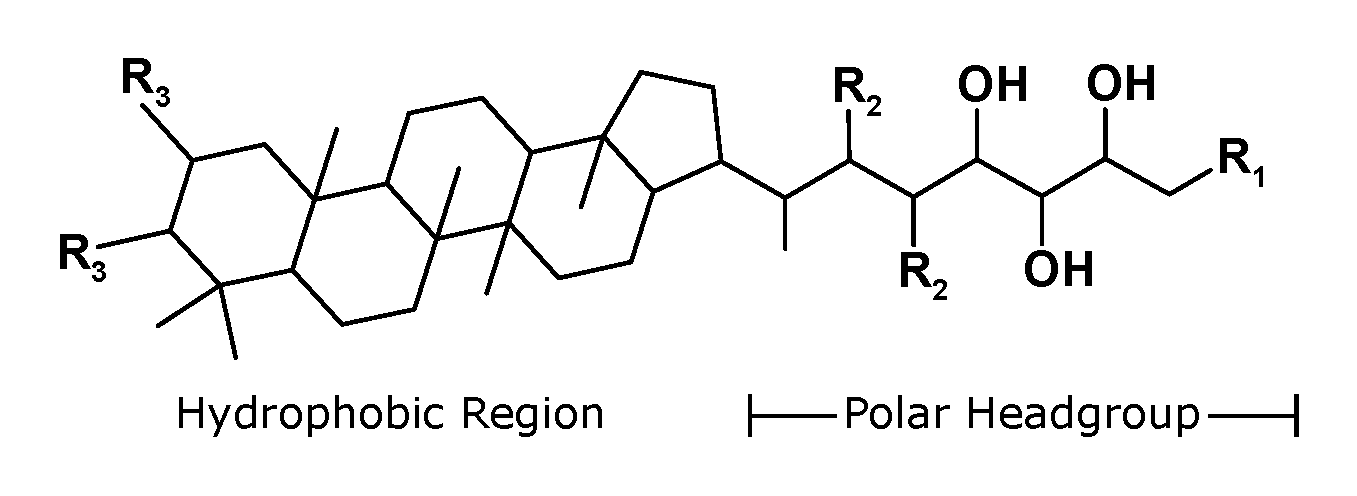
\includegraphics[width=1\linewidth]{figs_ch3/BHP_structure_general.pdf}
\caption[Generalized bacteriohopanepolyol chemical structure]{Generalized bacteriohopanepolyol (BHP) chemical structure. For BHPs without composite groups, R\textsubscript{1} represents a hydroxyl (OH), amine (NH\textsubscript{2}), or amminium (NH\textsubscript{3}\textsuperscript{+}) group. R\textsubscript{2} stands for H or OH. The BHP is considered pentafunctional if one R\textsubscript{2} is OH, or hexafunctional if both are OH. R\textsubscript{3} stands for H or CH\textsubscript{3}.}
\label{fig:BHP_structure}
\end{figure}
\doublespace




\singlespace
\begin{figure}[h]
\centering
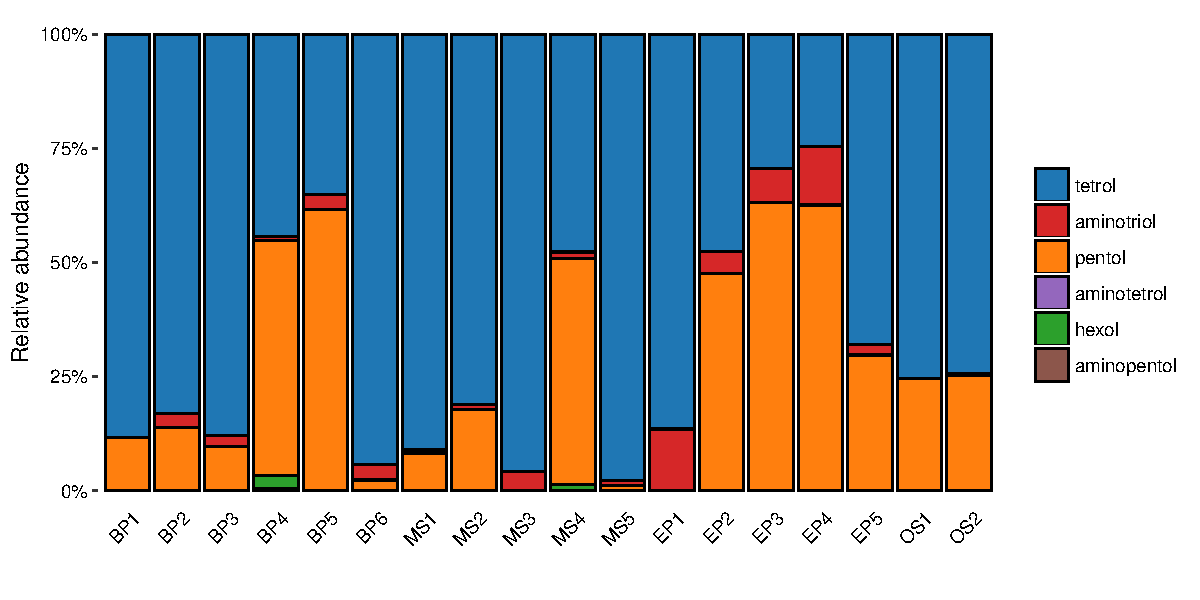
\includegraphics[width=1\linewidth]{figs_ch3/BHP_barchart.pdf}
\caption[Relative abundances of BHP polar headgroup functionality observed in Yellowstone hot spring sediments and biofilms]{Relative abundances of BHP polar headgroup functionality observed in Yellowstone hot spring sediments and biofilms.}
\label{fig:BHP_abund_Bison}
\end{figure}
\doublespace



\singlespace
\begin{figure}[h]
\centering
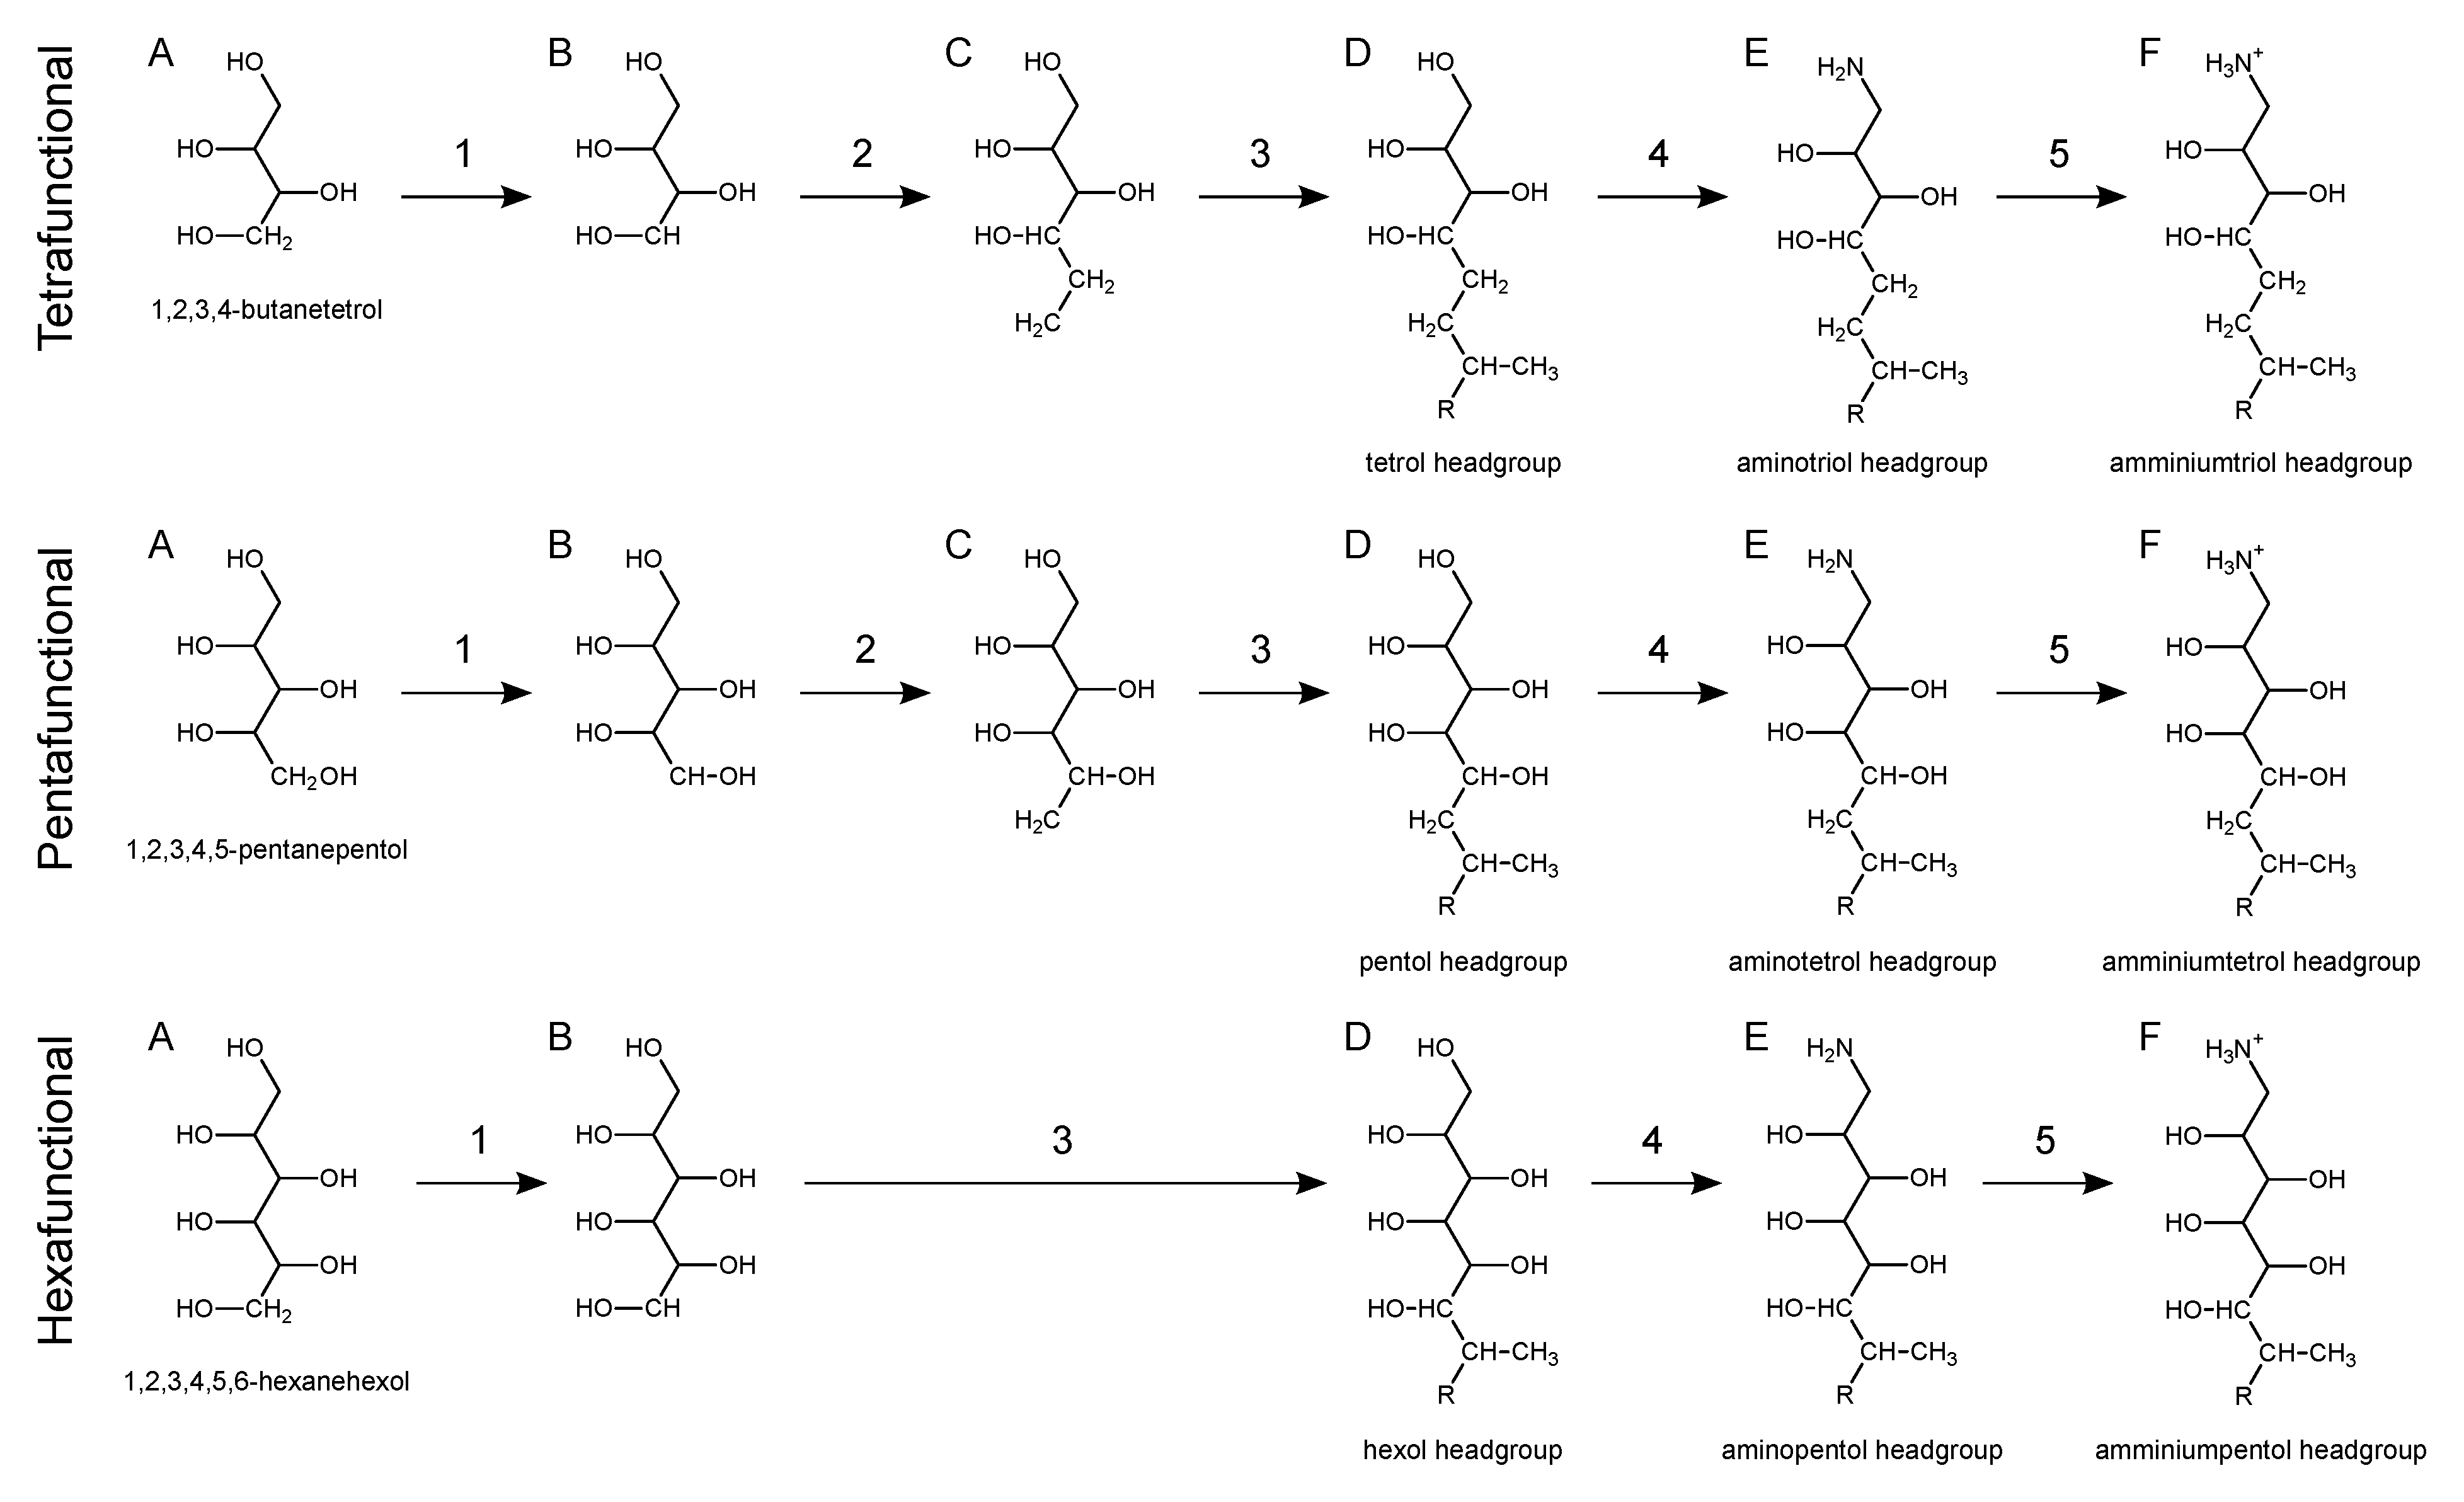
\includegraphics[width=1\linewidth]{figs_ch3/BHP_thermoest_paper.pdf}
\caption[Workflow used in the estimation of partial molal standard state thermodynamic properties of aqueous BHP headgroups]{Workflow used in the estimation of partial molal standard state thermodynamic properties of aqueous BHP headgroups. Structures and steps are described in the methods. R stands for the rest of the BHP structure, though its thermodynamic properties are not considered in this study.}
\label{fig:BHP_thermoest_paper}
\end{figure}
\doublespace


\singlespace
\begin{figure}[h]
\centering
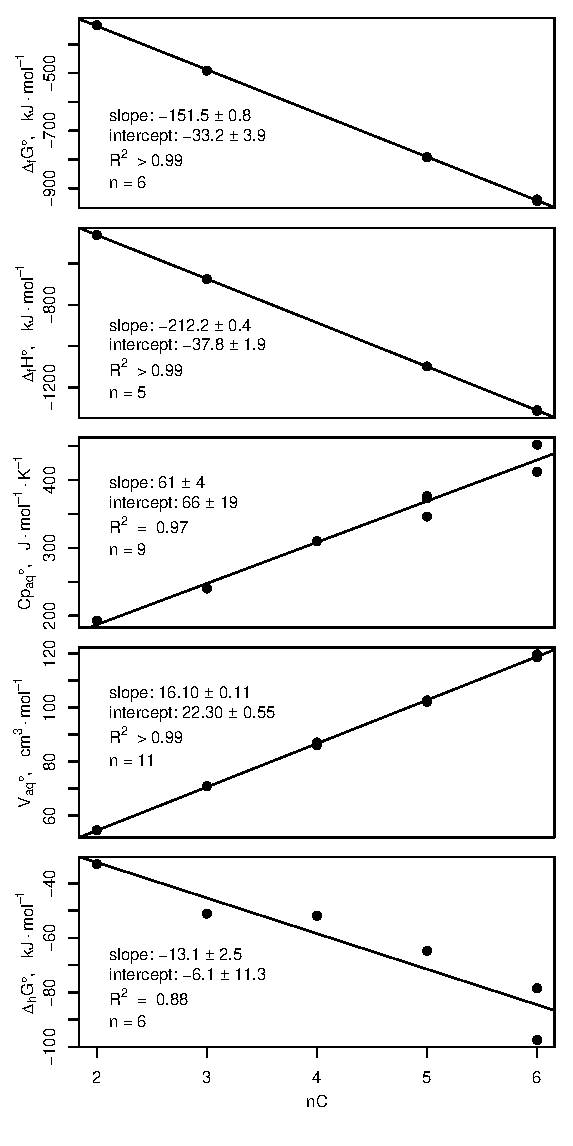
\includegraphics[width=0.5\linewidth]{figs_ch3/polyol_prop_regress.pdf}
\caption[Linear regression of experimentally-derived aqueous partial molal thermodynamic properties of sugar alcohols as a function of carbon length]{Linear regression of experimentally-derived aqueous partial molal thermodynamic properties of sugar alcohols as a function of carbon length (nC). Numbers of regressed datapoints for each plot are displayed equal to `n'. Literature sources for regressed data are given in Table \ref{tab:sug_alc}.}
\label{fig:polyol_prop_regress}
\end{figure}
\doublespace


\singlespace
\begin{figure}[h]
\centering
    \begin{subfigure}[b]{\linewidth}
        \includegraphics[width=\linewidth]{figs_ch3/"Bison OF1_BHP_mosaic"}
        \label{fig:BP1_degform}
    \end{subfigure}
    \begin{subfigure}[b]{\linewidth}
        \includegraphics[width=\linewidth]{figs_ch3/"Bison OF2_BHP_mosaic"}
        \label{fig:BP2_degform}
    \end{subfigure}
\end{figure}

\newpage

\begin{figure}[h]\ContinuedFloat
    \begin{subfigure}[b]{\linewidth}
        \includegraphics[width=\linewidth]{figs_ch3/"Bison OF3_BHP_mosaic"}
        \label{fig:BP3_degform}
    \end{subfigure}\\[-4ex]
    \begin{subfigure}[b]{\linewidth}
    	\includegraphics[width=\linewidth]{figs_ch3/"Bison OF4_BHP_mosaic"}
        \label{fig:BP4_degform}
    \end{subfigure}
\end{figure}

\newpage

\begin{figure}[h]\ContinuedFloat
    \begin{subfigure}[b]{\linewidth}
        \includegraphics[width=\linewidth]{figs_ch3/"Bison OF5_BHP_mosaic"}
        \label{fig:BP5_degform}
    \end{subfigure}
    \begin{subfigure}[b]{\linewidth}
        \includegraphics[width=\linewidth]{figs_ch3/"Bison OF6_BHP_mosaic"}
        \label{fig:BP6_degform}
    \end{subfigure}\\[-4ex]

\caption[lot cap]{cap}
\label{fig:degree_formation_bison}
\end{figure}
\doublespace




\singlespace
\begin{figure}[h]
\centering
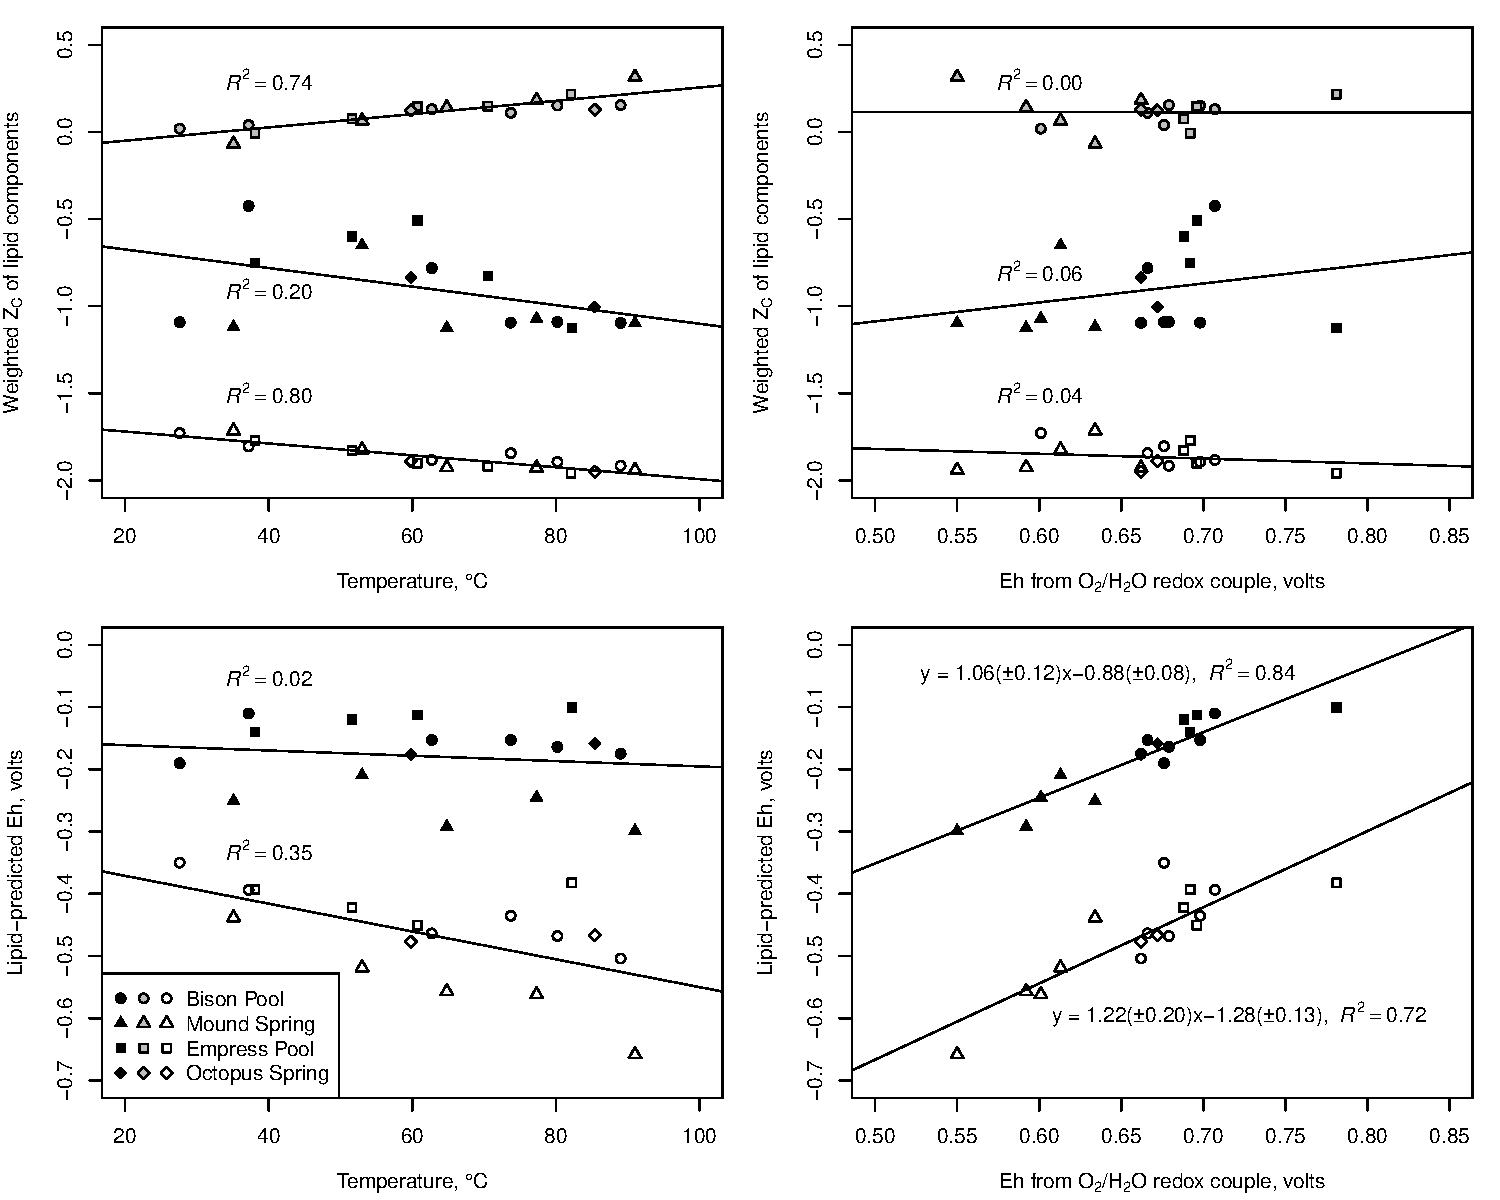
\includegraphics[width=1\linewidth]{figs_ch3/ZC_Eh_fourpanel.pdf}
\caption[Weighted Z\textsubscript{C} of thermophile lipid components and lipid-predicted Eh as a function of temperature and redox potential]{Weighted Z\textsubscript{C} of thermophile lipid components and lipid-predicted Eh as a function of temperature and redox potential. Black and gray symbols indicate headgroups of BHPs and IPLs, respectively. White/empty symbols indicate IPL alkyl chains in the upper plots or site-averaged IPL alkyl chains in the lower plots. Values for Z\textsubscript{C} of IPL components and alkyl chain-predicted Eh are taken from \cite{boyer2018thermophile} and \cite{boyer2018thermodynamic}, respectively. Standard errors of slopes and intercepts of linear fits are shown in parentheses and do not include propagated uncertainties from underlying thermodynamic estimations. Unweighted linear models were used to generate R\textsuperscript{2} values.}
\label{fig:ZC_Eh_fourpanel}
\end{figure}
\doublespace